% !TeX spellcheck = en_US
%Publications.tex
%\newcommand{\PublicationsPath}{PatentsAndPublications/Publications}

%BMSB2018

\section[MEC Proxy for efficient cache and reliable multi-CDN video distribution]{MEC Proxy for efficient cache and reliable multi-CDN video distribution}
\label{chap:BMSB2018}
\begin{itemize} \itemsep1pt\parskip0pt\parsep0pt
	\item \textbf{Title:} MEC Proxy for efficient cache and reliable multi-CDN video distribution
	\item \textbf{Authors:} Roberto Viola, \'Angel Mart\'in, Mikel Zorrilla and Jon Montalb\'an
	\item \textbf{Proceedings:} 2018 IEEE International Symposium on Broadband Multimedia Systems and Broadcasting (BMSB)
	\item \textbf{Publisher:} IEEE
	\item \textbf{Year:} 2018
	\item \textbf{DOI:}  \url{10.1109/BMSB.2018.8436904}
\end{itemize}	

\textbf{Abstract:} The massive consumption of media contents needs of network accelerators, which boost the media delivery and optimize the traffic volume crossing the network from servers to media players. Content Delivery Network (CDN) is the common network function to distribute in a cloud-manner the contents, enhancing media availability and distribution performance. However, high concurrency rates of media sessions can produce CDN performance degradations and outages that impact negatively the Quality of Experience (QoE). 5G Multi-access Edge Computing (MEC) architecture envisions a QoE-aware system at the network edge which performs analytics to enhance or boost media services. This paper provides a novel MEC proxy to expand and enforce caching infrastructures for efficient and reliable content distribution. First, the proxy caches contents on the network edge to reduce the Capital Expenditure (CAPEX) of the CDN for the OTT service provider. To this end, the proxy is able to identify recurrent requests. Second, the proxy shields from identified or predicted CDN malfunction. Here, the proxy switches the download sessions to an alternative CDN in order to ensure QoE rates, enabling a CDN dynamic selection based on live connectivity statistics. The proposed solution is evaluated by delivering Dynamic Adaptive Streaming over HTTP (MPEG-DASH) streams in a dense client cell while applying different caching strategies.

\textbf{Keywords:} 5G, CDN, distributed cache, MEC, QoE, reliability \& streaming analytics.	
	
	
\subsection{Introduction}

The increase of video streaming users and the service requirements are driving the evolution of media services over the Internet. Mobility and quality improvements are the key catalysers in this evolution. Cisco estimates that video traffic will cover the 82\% of all Internet traffic by 2021 \cite{ciscovideo2016}. Moreover, mobile traffic growth is estimated to be twice as fast as fixed IP traffic from 2016 to 2021 \cite{ciscomobile2016}.

The delivery performance from the network has a big impact on the perceived QoE of the end user of media services. However, video streaming services work on top of unmanaged networks, where the traffic is managed and forwarded on a best-effort basis \cite{sodagar2011mpeg}. This operational context is targeted by the video streaming solution MPEG-DASH. MPEG-DASH inherits many benefits from Hypertext Transmission Protocol (HTTP). First, it enables a pull-based streaming \cite{begen2011} to easily traverses network functions such as firewalls and NAT devices. Second, MPEG-DASH streams can be played anywhere as any connected device supports HTTP. Third, MPEG-DASH has a Content Delivery Network (CDN)-ready design enabling the exploitation of existing HTTP caching infrastructures, which enhance the availability and the responsiveness of the content distribution.

Beyond the current network functions to boost and enhance the traffic delivery, the capacity and performance promised by 5G networks will make a significant leap towards higher data rates, heavier user densities and ultra-reliable and low-latency communications. The European Telecommunications Standards Institute (ETSI) specifies a set of component technologies which will be essential part of 5G systems, such as, Network Functions Virtualization (NFV), Millimetre Wave Transmission (mWT), Next Generation Protocols (NGP) and Multi-access Edge Computing (MEC) \cite{etsi2019}. MEC architecture allows Mobile Network Operators (MNOs) to supply video delivery analytics-based intelligence at the network edge. Thus, MEC plays a significant role to achieve specific media traffic goals with zero-latency in a distributed manner. Furthermore, MEC enables coordinated operations at the network edge such to be transparent to the media server and players.

This work proposes a novel network proxy, called MEC4CDN, which complies with MEC architecture. MEC4CDN provides two features. First, it performs a local cache of identified trending contents to minimize the traffic between the CDN and the network edge. Second, it applies a dynamic selection of the CDN based on live measurements in the context of a multi-CDN delivery. The proposed solution allows the client to start playing from a CDN, that is favourable in terms of Quality of Service (QoS), and transparently and dynamically switch to another one which provides better performance in case of CDN degradation or outage. To this end, the proxy collects and process L3 connectivity metrics, L7 MPEG-DASH Media Presentation Description (MPD) files and L7 QoE scores. So, the proxy handles multiple CDN endpoints, deciding to locally cache a response for near future requests, or to conduct the request to a healthy cloud CDN in case of detected issues.

The paper is structured as follows. First, section \ref{sec:BMSB2018related} reviews the related work to improve the network delivery. Then, section \ref{sec:BMSB2018multi-CDN} describes the proposed MEC4CDN network proxy. Section \ref{sec:BMSB2018implementation} presents the implementation of the solution. To validate the solution, section \ref{sec:BMSB2018results} compiles the testbed and the results. Finally, section \ref{sec:BMSB2018conclusion} gathers the conclusions of this work.

\subsection{Related Work}
\label{sec:BMSB2018related}

Apart from the content catalogue, the Quality of Experience (QoE) is a key aspect for user satisfaction and retention when rating streaming services. Hence, any system trying to enhance media delivery needs to consider QoE metrics.

QoS assesses the network delivery performance and it has a direct impact on human perception QoE. In this sense, stability of media playback is related to efficient utilization and fair resource sharing. Nevertheless, these key aspects are not guaranteed in unmanaged networks. This situation may lead to suboptimal results in terms of video playback, link utilization, and fairness among the clients \cite{chen2016}. 

Specific metrics for QoE of HTTP-based adaptive media streaming services, such as initial delay, stalling time, number of quality switches and inter-switching times, are fundamental parameters to get the estimated Mean Opinion Score (eMOS) \cite{claeys2014}. This model quantifies the quality of video streaming services without a demographic perception study. Recently, the work \cite{lentisco2017} investigates a new model for MOS, called Ubiquitous-Mean Opinion Score for Video (U-vMOS), which makes initial buffering more dominant than \cite{claeys2014} model.

Caching is a common technique to get enhanced QoE for massive content consumption services. The CDN is the traditional network function provisioning cache features as a cloud service. Fueled by the CDN vendor proliferation, media services employ multi-CDN strategies to get a more reliable and cost-effective content delivery. Netflix case, as an example of multi-CDN solution, is studied in \cite{adhikari2012}. More recent work \cite{adhikari2015} also includes Hulu analysis for 3 CDN vendors. Here, with alternative CDNs available, the employed CDN is set by the streaming service for each session, where the choice is done by the server. This centralized architecture is difficult to scale hampering the orchestration of common policies or decisions to all users in an area.

When the employed CDN is not pre-set, transferring to clients the possibility to dynamically choose, each client should analyze repeatedly the network performance of each CDN. It means the introduction of a network overhead proportional to the number of clients and the number of CDNs. Hence, a client-side CDN selection is not an optimal solution.

Consequently, the European Broadcasting Union (EBU) aims to avoid both pre-set CDN and client's CDN selection by proposing the EBU Flow Multi-CDN \cite{EurovisionFLOW}. It consists in a CDN switching service which selects the optimal CDN at any given moment in time. A similar solution is also provided by Cedexis Multi-CDN \cite{cedexis}. Both EBU and Cedexis proposals monitor network analytics at core network, then they are not aware of the state of connected clients at network edge.

On the contrary, if we focus at the network edge, the access point has knowledge of both the connected clients' activity in its cell and the CDN performance from its location. A proxy located at the network edge, retrieving access point information, can evaluate the performance of the delivery network just once and exploit it for each client (independently from the number of clients in the cell). This perfectly suits the telecommunication industry which proposes MEC as a new functional architecture to be integrated on the mobile network infrastructure. MEC allows Internet service provider (ISP) to provide Information Technology (IT) and cloud computing services at the edge of the network, closer to the clients. Hence, MEC opens the door for authorized Content Providers (CPs) to develop their own applications hosted on the MEC server. Therefore, CPs are able to tune the behavior of content delivery to end users in 4G and 5G contexts. Furthermore, next generation networks and 5G MEC architecture enable the deployment of distributed local caches at the network edge to efficiently minimize the volume of traffic passing through the network core and backhaul.

\subsection{MEC Proxy for Multi-CDN Delivery}
\label{sec:BMSB2018multi-CDN}

The proposed MEC4CDN proxy server, located on a MEC component, can exploit the knowledge of network analytics of different delivery paths. It aims to improve the overall throughput while minimizing the latency, in an environment where multiple clients are competing for network resources. 

Figure \ref{fig:BMSB2018selection} shows a scenario where a content is provided by means of two CDN vendors. For some reasons, such as sudden massive connections or geo-based cycles of human activity, the performance of \textit{CDN A} starts to degrade. At the same time, the capacity of \textit{CDN B} is improved because the \textit{CDN B} starts to provision more resources for a specific area. The MEC4CDN system gets awareness of this unbalanced situation, based on L3 stats, and orchestrates all the media players subscribed to the managed cell to dynamically employ a CDN which ensures better QoS. 

\begin{figure}[htp]
	\centering
	\includegraphics[width=1\textwidth,keepaspectratio]{selection.pdf}
	\caption{MEC4CDN multi-CDN selection.}
	\label{fig:BMSB2018selection}
\end{figure}

Therefore, for services delivered over multiple CDN providers, MEC4CDN can select an appropriate CDN for a RAN geo-position in real-time, according to L3 metrics. To this end, MEC4CDN gets alternative CDNs set from the MPD file, provided that it contains multiple definitions of \textit{base URL} storing the path to the CDNs, or from the media service. Then, MEC4CDN employs the set of CDNs to dynamically switch the base URL of media sessions in the same RAN when necessary. So, in case of detected performance degradation, the MEC4CDN system replaces the base URL field of all the managed sessions to another known CDN endpoint, migrating all the managed clients at once to avoid outages.

The sequence diagram with the exchanged messages to allow the CDN switching is depicted in Figure \ref{fig:BMSB2018sequence_cdn}. First, the MEC proxy server running MEC4CDN captures the HTTP GET requests from the User Equipments (UEs) to download the MPD file from the media server. Then, MEC4CDN retrieves the MPD file from the media server and appropriately parses it in order to retrieve the \textit{base URLs} set before sending it to the UE. Then, the UE selects a representation bitrate ($R_j$) from the available ones according to display resolution, user preferences and connection capacity stats. The UE requests, through the MEC proxy, a specific segment file to the CDN accordingly. Once the MEC proxy server detects the HTTP GET requests from the UEs for downloading a segment file, it retrieves wired path stats. When network performance is not enough, the MEC4CDN switches the \textit{base URL} field of the MPD file applicable for the next segment requests. Such operations are executed at the stream start and each time that the UEs asks for a new segment.

\begin{figure}[htp]
	\centering
	\includegraphics[width=1\textwidth,keepaspectratio]{sequence_cdn_healthy.png}
	\caption{MEC4CDN multi-CDN sequence diagram.}
	\label{fig:BMSB2018sequence_cdn}
\end{figure}

Furthermore, MEC4CDN ships the ability to significantly reduce the CDN traffic for a live content distribution in dense client cells, as depicted in Figure \ref{fig:BMSB2018cache}. In a live media consumption scenario, each UE makes a request to get the video from a CDN. When MEC4CDN comes into play, it performs a local cache at the network edge in a proactive manner. Triggered by the first content request, MEC4CDN downloads all the next segment representations from the CDN. Then, all the following requests are already downloaded and available in the MEC4CDN local cache for any representation bitrate chosen by the media players. Then, the greater the number of clients consuming a live content in a cell, the higher efficiency of this solution.

\begin{figure}[htp]
	\centering
	\subfloat[]
	{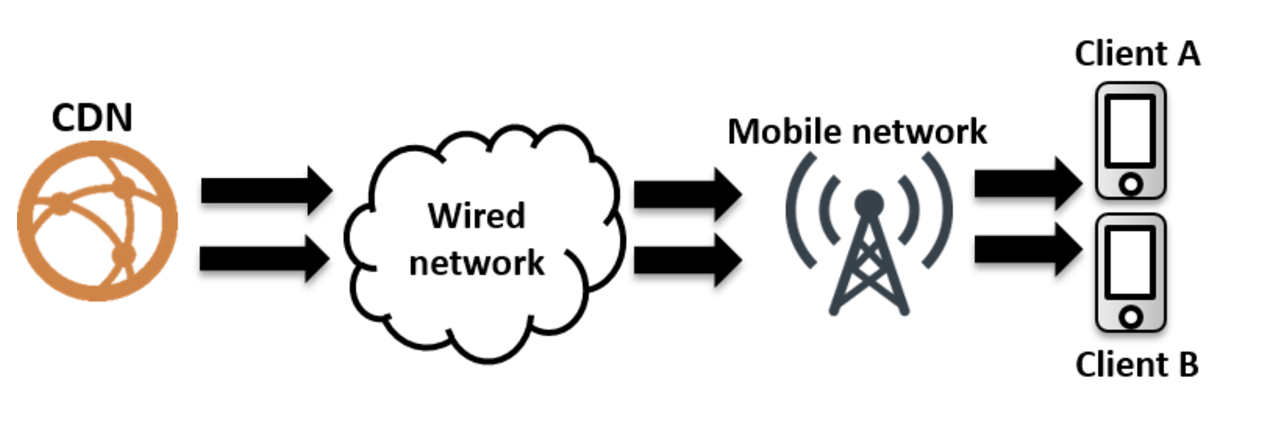
\includegraphics[width=0.8\textwidth,keepaspectratio]{legacy-cache.eps}
		\label{fig:BMSB2018legacy-cache}
	}
	\hfil
	\subfloat[]
	{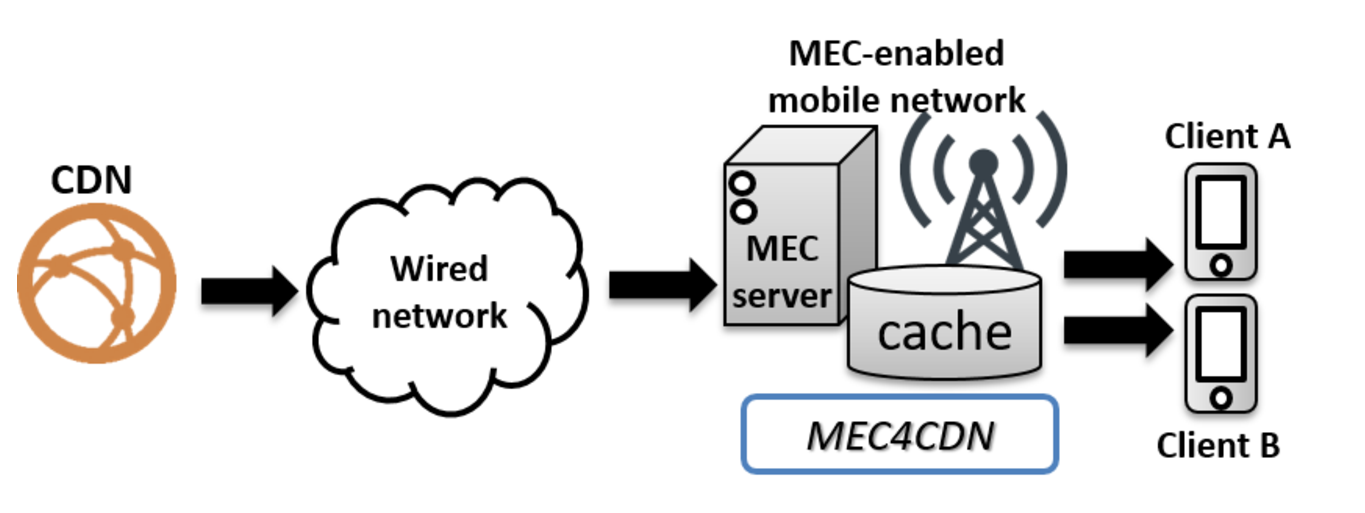
\includegraphics[width=0.8\textwidth,keepaspectratio]{cache.eps}
		\label{fig:BMSB2018cache}
	}
	\hfil
	\caption{Legacy content delivery (a) and MEC4CDN cache-powered delivery (b).}
\end{figure}


The utilization of a CDN means a significant operational cost for media services. Moreover, when massive connections come concurrently to a CDN, the CDN infrastructure can start to collapse and the QoS could be negatively impacted. To prevent media delivery from this situation, it is necessary to turn broadcast of live content into an efficient distribution. To this end, MEC systems located at the network edge can cache recurrent contents, such as live sports events or concerts, in a proactive manner. Cache at network edge can improve the streaming experience caching all available representations. Thus, the selected representation will be locally available for any number of subscribers in a cell, enabling the video to start faster and reducing the buffering time, while minimizing CDN traffic. This approach preserves media players ability to decide the bitrate that fits with their contexts independently.

The sequence diagram with the exchanged messages to allow the local cache of a popular or live content is depicted in Figure \ref{fig:BMSB2018sequence_cache}. The proxy waits for a media content request and proceeds to download all the available representations. Then, the media players in the cell will select a specific representation ($R_j$) according to the device features, the assessed available bandwidth, the user preferences and subscription plan. Once the players start to request a representation for a specific time ($t$), the proxy requests the next segments ($Segments_{t+1} \forall R_j$) to be ready for the following requests.

\begin{figure}[htp]
	\centering
	\includegraphics[width=1\textwidth,keepaspectratio]{sequence_cache.png}
	\caption{MEC4CDN cache sequence diagram.}
	\label{fig:BMSB2018sequence_cache}
\end{figure}

It is also important to remark the zero-latency and distributed performance features by design coming from the MEC architecture fundamentals. The MEC systems are distributed and autonomously empower specific services for the co-located cell.

\subsection{Implementation}
\label{sec:BMSB2018implementation}

\makeatletter
\newlength{\trianglerightwidth}
\settowidth{\trianglerightwidth}{$\triangleright$~}
\algnewcommand{\LineComment}[1]{\Statex \hskip\ALG@thistlm $\triangleright$ #1}
\algnewcommand{\LineCommentCont}[1]{\Statex \hskip\ALG@thistlm%
	\parbox[t]{\dimexpr\linewidth-\ALG@thistlm}{\hangindent=\trianglerightwidth \hangafter=1 \strut$\triangleright$ #1\strut}}
\renewcommand{\ALG@beginalgorithmic}{\small}
\makeatother

The program of MEC4CDN for CDN selection is described in Algorithm \ref{alg:BMSB2018algorithmCDN}. The outcome of MEC4CDN is to identify violations of bandwidth or latency performance in order to perform reactive switching to an alternative CDN provider. The inputs of the algorithm are the RTT and the bandwidth from the MEC4CDN proxy to the CDN and the current number of media playing sessions to this CDN. The output is the base URL field of the updated MPD file to be used by the media player.

\begin{algorithm}
	\renewcommand{\algorithmicrequire}{\textbf{Input:}}
	\renewcommand{\algorithmicensure}{\textbf{Output:}}
	\caption{CDN health check to switch all sessions at eNodeB}
	\label{alg:BMSB2018algorithmCDN}
	\begin{algorithmic}
		
		\Procedure{CDNcheck}{ } \Comment{\parbox[t]{.30\linewidth}{listen to requests \& switch CDN}}
		\State rtt$_{max}$ \Comment{setup maximum latency}
		\State CDN$_{list}$ \Comment{set of alternative CDNs}
		\State n$_{p}$ \Comment{number of players}
		\ForAll {segment request} \Comment{from the UE}
		\State SegmentRequest() \Comment{to the CDN$_\textit{k}$}
		\State s$_{CDN_\textit{k}}$ $\leftarrow$ SegmentResponse() \Comment{from the CDN$_\textit{k}$}
		\State rtt$_{CDN_\textit{k}}$ $\leftarrow$ rtt(s$_{CDN_\textit{k}}$) \Comment{L3 latency}
		\State bw$_{CDN_\textit{k}}$ $\leftarrow$ 2$\frac{size(s_{CDN_\textit{k}})}{rtt(s_{CDN_\textit{k}})}$ \Comment{L3 BW}
		\State R$_{max}^{bitrate}$ $\leftarrow$ parse(MPD) \Comment{\parbox[t]{.25\linewidth}{maximum representation bitrate}}
		\If {(rtt$_{CDN_\textit{k}}$ $>$ rtt$_{max}$) $||$ (bw$_{CDN_\textit{k}}$ $<$ (n$_{p}$ x R$_{max}^{bitrate}$))} 
		\State \Comment{insufficient performance}
		\State baseURL $\leftarrow$ alternative(CDN$_{list}$,$CDN_{k}$)
		\State \Comment{change CDN}
		\EndIf
		\EndFor
		\EndProcedure
	\end{algorithmic}
\end{algorithm}

Moreover, the program of MEC4CDN for local cache is described in Algorithm \ref{alg:BMSB2018algorithmCache}. The outcome of MEC4CDN is to proactively download what the users will play in order to locally cache next segments before the player needs to play them, enabling the video to start faster, decreasing stalls, reducing CDN traffic and enhancing the quality of experience. Thus, MEC4CDN reduces resource usage coming from the CDN provider by caching requested contents and exploiting their recurrent likelihood. The inputs of the algorithm are the current segment index employed by the media player and the available representations. The result is the temporal storage of next segments to be requested beyond the current one played by the user.

\begin{algorithm}
	\renewcommand{\algorithmicrequire}{\textbf{Input:}}
	\renewcommand{\algorithmicensure}{\textbf{Output:}}
	\caption{Cache proxy at eNodeB}
	\label{alg:BMSB2018algorithmCache}
	\begin{algorithmic}
		
		\Procedure{LocalCache}{ } \Comment{\parbox[t]{.27\linewidth}{listen to requests \& cache segments}}
		\State i$_{t}$ \Comment{current segment index}
		\State \{R$_{j}$\} \Comment{set of alternative representations}
		\ForAll {R$_j$ $\in$ \{R$_{j}$\}} \Comment{download next segment}
		\State s$_{i_{t}+1}$ $\leftarrow$  Download(i$_{t}+1$,R$_j$) \Comment{from the CDN}
		\State Cache(s$_{i_{t}+1}$,R$_j$) \Comment{at eNodeB proxy}
		\EndFor
		\EndProcedure
		
	\end{algorithmic}
\end{algorithm}


\subsection{Results}
\label{sec:BMSB2018results}

In order to test MEC4CDN solution, we deploy an experimental setup by exploiting a MPEG-DASH distributed dataset described by Lederer et al. \cite{lederer2013} and provided for public experimentation of CDN-like infrastructures. This dataset consists in Red Bull Playstreet sequence stored at several geographically distributed mirror servers. The content is provided in 17 video representations encoded in H.264 Advanced Video Coding (H.264/AVC) and 4 dual channel audio representations encoded in Advanced Audio Coding (AAC). Both audio and video are segmented with different segment lengths of 2, 4, 6, 10, and 15 seconds and multiplexed in ISO MPEG4 files (ISO/IEC 14496-12 - MPEG-4 Part 12).

\begin{table}[htp]
	\caption{Set of MPEG-DASH representations employed in the experiments.}
	\centering
	\bgroup
	\def\arraystretch{1.2}%  1 is the default, change whatever you need
	\setlength\tabcolsep{2.5pt} % default value: 6pt
	\label{tab:BMSB2018reps}
	{\scriptsize
		\begin{tabular}{>{\centering\arraybackslash}m{\dimexpr0.1\textwidth-2\tabcolsep-\arrayrulewidth\relax}
				>{\centering\arraybackslash}m{\dimexpr0.15\textwidth-2\tabcolsep-\arrayrulewidth\relax}
				>{\centering\arraybackslash}m{\dimexpr0.15\textwidth-2\tabcolsep-\arrayrulewidth\relax}
				>{\centering\arraybackslash}m{\dimexpr0.15\textwidth-2\tabcolsep-\arrayrulewidth\relax}
			}
			\toprule
			\textbf{index} & \textbf{bitrate} & \textbf{resolution} & \textbf{framerate} \\
			\midrule
			\midrule
			1 & 400kbps & 480x360 & 30fps  \\
			2 & 900kbps & 854x480 & 30fps  \\
			3 & 1500kbps & 1280x720 & 30fps \\
			4 & 2000kbps & 1280x720 & 30fps \\
			5 & 2500kbps & 1280x720 & 30fps \\
			6 & 3000kbps & 1920x1080 & 30fps \\
			\bottomrule
			\bottomrule
		\end{tabular}
	}
	\egroup
\end{table}

Then, the overall experimental setup comprises both public network nodes and internal ones belonging to our network infrastructure:
\begin{itemize}
	\item Three mirror servers: network nodes provided by Lederer et al. \cite{lederer2013} which we use as CDN-like nodes for storing the media segments.
	\item A media server: a server in our infrastructure storing the MPD file which is requested by the client to play the content.
	The MPD file provides information for the player to retrieve the segments from the mirror servers. Moreover, the service employs segments with duration of 6 seconds and the video content is limited to six different representations, widely used by market services. Each representation is characterized by a specific bitrate as shown in Table \ref{tab:BMSB2018reps}.
	\item A proxy server running MEC4CDN: a server in our infrastructure provided by public Internet connection and acting as a network gateway for the wireless network edge deployed inside our infrastructure. Then, all the requests from the players are processed by the proxy server before being transmitted, if necessary, to the media infrastructures on Internet. It executes the proposed MEC4CDN solution. 
	\item A wireless access point: in order to provide wireless capabilities, an access point is used, which provides a wireless local area network (WLAN) using 2.4Ghz band. The access point is directly connected to the proxy server to provide a MEC-like architecture. The only role of the access point consists in forwarding all the incoming traffic on both directions (download and upload).
	\item A UE running MPEG-DASH players: a wireless network node connected to the access point, which is running GStreamer MPEG-DASH players.
\end{itemize}
The experimental setup is shown in Figure \ref{fig:BMSB2018testbed}.

\begin{figure}[htp]
	\centering
	\includegraphics[width=1\textwidth,keepaspectratio]{testbed2.pdf}
	\caption{Testbed.}
	\label{fig:BMSB2018testbed}
\end{figure}

The tests include two different experiments aiming to verify separately the two main features of MEC4CDN:
\begin{itemize}  
	\item Multi-CDN experiment: the proxy server running MEC4CDN employs a multi-CDN infrastructure which allows CDN malfunction detection and switches the content download to an alternative CDN when necessary. In order to simulate CDN malfunctions, we introduce a random latency between 0 and 500 milliseconds on the wired path between the MEC4CDN proxy and the three mirror servers storing the segments.
	\item Local cache experiment: the proxy server running MEC4CDN empowers the content delivery by caching segments at the network edge. This enables the reduction of CDN transactions, while improving the delivery with lower experienced latency.
\end{itemize}

In both experiments, 20 players are sharing both core and network edge resources, competing for the shared wireless access point. The duration of each experiment is fixed to 10 minutes.

Moreover, to get evidence of the benefits of MEC4CDN solution, we carry out the two mentioned experiments where MEC4CDN comes into play and a baseline one without MEC4CDN. This basic setup provides a common delivery infrastructure where the network just forwards the requests to the first CDN. Here, GStreamer players are not able to identify CDN malfunctions, then they use always the same pre-set CDN even when it is suffering severe latency issues. Moreover, no cache is done at the edge, which means that CDN bandwidth is shared among the concurrent clients.


\begin{figure}[htp]
	\centering
	\subfloat[]{\includegraphics[width=1\textwidth,clip,keepaspectratio]{switch_legacy-cdn.pdf}%
		\label{fig:BMSB2018experiments1c}}
	\hfil
	\subfloat[]{\includegraphics[width=1\textwidth,clip,keepaspectratio]{switch_cdn.pdf}%
		\label{fig:BMSB2018experiments1d}}
	\hfil
	\caption{Representation selection over time: legacy CDN (a) and MEC4CDN multi-CDN (b).}
	\label{fig:BMSB2018experiments1}
\end{figure}

Concerning the first experiment, Figure \ref{fig:BMSB2018experiments1} shows the representation switches along the multi-CDN experiment (10 minutes) where principal CDN suffers performance degradation. In Figure \ref{fig:BMSB2018experiments1c} the actors are not able to take decisions while in Figure \ref{fig:BMSB2018experiments1d} MEC4CDN apply strategies to switch to a healthy CDN. It is clear from the graphs that a legacy solution (\ref{fig:BMSB2018experiments1c}) does not let the players to continue playing at the same representation level when a malfunction occurs while downloading the content. The players reduce the chosen representation bitrate in order to continue playing. In the case of a multi-CDN strategy (\ref{fig:BMSB2018experiments1d}), some players access to higher representation bitrates since the MEC4CDN is able to enforce the delivery by switching to another CDN which better performs.

The improvements are also evident by the eMOS evaluation. The eMOS mean value among all the clients is 3.09 while downloading from a single CDN and 3.47 in case of multi-CDN delivery. This means a eMOS enhancement of +12.3\%.

\begin{figure}[htp]
	\centering
	\subfloat[]{\includegraphics[width=1\textwidth,clip,keepaspectratio]{bitrate_legacy-cache.pdf}
	\label{fig:BMSB2018experiments2a}}
	\hfil
	\subfloat[]{\includegraphics[width=1\textwidth,clip,keepaspectratio]{bitrate_cache.pdf}
	\label{fig:BMSB2018experiments2b}}
	\hfil
	\caption{Mean value and deviation of measured bitrate and selected representation bitrate: legacy content delivery (a) and MEC4CDN cache-powered content delivery (b).}
	\label{fig:BMSB2018experiments2}
\end{figure}

Regarding the second experiment, Figure \ref{fig:BMSB2018experiments2} shows the mean value and the deviation of the measured bitrate and the representation bitrate. The results for a legacy content delivery are shown in Figure \ref{fig:BMSB2018experiments2a} and, when MEC4CDN with local cache delivery is added, the results improve as depicted in Figure \ref{fig:BMSB2018experiments2b}. 
This is clear since the cache lets the player to experience lower latency since the segments are closer to the clients, then the throughput is higher. Therefore, the clients tend to request higher representation bitrate which improves the user's QoE. 

In this case, the eMOS mean value among all the clients is 3.08 in case of legacy delivery and 3.92 in case of cache-powered delivery, which means an eMOS increase of +27.3\%.


\subsection{Conclusion}
\label{sec:BMSB2018conclusion}
This paper proposes a network proxy which enables multi-CDN video distribution and local cache at the network edge by exploiting the MEC architecture proposed by ETSI for future 5G networks.

The proposed proxy has two main outcomes. First, the proxy reduces the CAPEX of the CDN since it makes distributed cache at the network edge, then all the clients can play the contents received from the cache. Second, the proxy shields from CDN malfunction by switching the content download session to another available CDN such to keep QoE rates.

Finally, this proposal has been tested by performing two experiments on a real testbed. The first one exploiting a multi-CDN delivery and the second one employing local cache at network edge. In both the experiments, the results show that the MPEG-DASH players experience higher QoE compared to a legacy content delivery.



%\subsection*{Acknowledgment}

		
